\documentclass[../mathNotesPreamble]{subfiles}
\begin{document}
%\relscale{1.4}
\section{6.1: Velocity and Net Change}

  \begin{defn*}[Position, Velocity, Displacement, and Distance]
    \begin{enumerate}
      \item 
        The \textbf{position} of an object moving along a line at time $t$, denoted $s(t)$, is the location of the object relative to the origin.
      \item 
        The \textbf{velocity} of an object at time $t$ is $v(t)=s'(t)$.
      \item 
        The \textbf{displacement} of the object between $t=a$ and $t=b>a$ is
          \[s(b)-s(a)=\int_a^b v(t)\,dt.\]
      \item 
        The \textbf{distance traveled} by the object between $t=a$ and $t=b>a$ is
          \[\int_a^b\abs{v(t)}\,dt\]
        where $\abs{v(t)}$ is the \textbf{speed} of the object at time $t$.
    \end{enumerate}
  \end{defn*}

  \vspace*{\stretch{1}}
  \begin{center}
    \includegraphics[width=0.325\linewidth, trim={0mm, 78.5mm, 0mm, 0mm}, clip]{../images/briggs_06_01/fig06_02}
    \hspace*{0.05\linewidth}
    \includegraphics[width=0.325\linewidth, trim={0mm, 0mm, 0mm, 95mm}, clip]{../images/briggs_06_01/fig06_02}
  \end{center}
  \vspace*{\stretch{1}}
  \pagebreak
  \begin{ex*}
    Suppose an object moves along a line with velocity (in ft/s) $v(t)=6-2t$, for $0\leq t\leq 5$, where $t$ is measured in seconds. 
  \end{ex*}
  \begin{itemize}[itemsep=\stretch{1}]
    \item 
      Find the displacement of the object on the interval $0\leq t\leq5$.
    \item 
      Find the distance traveled by the object on the interval $0\leq t\leq5$.
  \end{itemize}
  \vspace*{\stretch{1}}
  \begin{center}
    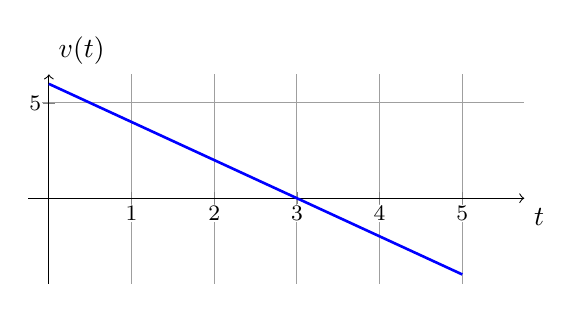
\begin{tikzpicture}
      \begin{axis}[
        grid=both, %major,minor
        grid style={line width=0.3pt, draw=gray!60},
        major grid style={line width=0.375pt, draw=gray!75},
        axis lines=center,
        axis line style={black,->},
        xmin=-0.25, xmax=5.75,
        ymin=-4.5, ymax=6.5,
        ticklabel style={font=\footnotesize,inner sep=0.5pt,fill=white,opacity=1.0, text opacity=1},
        xlabel=$t$, xlabel style={at={(ticklabel* cs:1)},anchor=north west},
        ylabel=$v(t)$, ylabel style={at={(ticklabel* cs:1)},anchor=south west},
        every axis plot/.append style={line width=0.95pt, color=blue, samples=100},
        width=0.65\linewidth, height=0.35\linewidth
        ]
         \addplot[-] expression[domain=0:5]{6-2*x};      
      \end{axis}
    \end{tikzpicture}
  \end{center}
  \pagebreak

  \begin{ex*}
    A cyclist rides down a long straight road at a velocity (in m/min) given by $v(t)= 400-20t$, for $0\leq t\leq 10$.
  \end{ex*}
  \begin{tasks}[after-item-skip=\stretch{1}, label=\textbullet](1)
    \task 
      How far does the cyclists travel in the first $5$ minutes?
    \task 
      How far does the cyclists travel in the first $10$ minutes?
    \task 
      How far has the cyclist traveled when her velocity is $250$ m/min?
  \end{tasks}
  \vspace*{\stretch{1}}
  \pagebreak

  \begin{ex*}
    The population of a community of foxes is observed to fluctuate on a 10-year cycle due to variations in the availability of prey.  When population measurements began ($t=0$), the population was $35$ foxes.  The growth rate in units of foxes/year was observed to be: 
  \end{ex*}
    \[P'(t)=5+10\sin\parens{\frac{\pi t}{5}}\]
  \begin{tasks}[after-item-skip=\stretch{1}, label=\textbullet](1)
    \task 
      Find $P(t)$.
    \task 
      Find the population of foxes after the first 5 years, rounded to the nearest whole number of foxes.
  \end{tasks}
  \vspace*{\stretch{1}}
  \pagebreak

  \vspace*{\stretch{0.75}}
  \begin{thmBox*}[Theorem 6.1: Position from Velocity]
    Given the velocity $v(t)$ of an object moving along a line and its initial position $s(0)$, the position function of the object for future times $t\geq 0$ is
      \[\underbrace{s(t)}_{\substack{\textnormal{position}\\ \textnormal{at $t$}}}=\underbrace{s(0)}_{\substack{\textnormal{initial}\\\textnormal{position}}}+\underbrace{\int_0^t v(x)\,dx}_{\substack{\textnormal{displacement}\\\textnormal{over $\sbrkt{0,t}$}}}.\]
  \end{thmBox*}
  \vspace*{\stretch{1}}

  \begin{thmBox*}[Theorem 6.2: Velocity from Acceleration]
    Given the acceleration $a(t)$ of an object moving along a line and its initial velocity $v(0)$, the velocity of the object for future times $t\geq 0$ is
      \[v(t)=v(0)+\int_0^t a(x)\,dx.\]
  \end{thmBox*}
  \vspace*{\stretch{1}}
  \pagebreak

  \begin{ex*}
    At $t=0$, a train approaching a station begins decelerating from a speed of $80$ miles/hour according to the acceleration function $a(t)=-1280(1+8t)^{-3}$, where $t\geq 0$ is measured in hours. The units of acceleration are mi/hr$^2$.
  \end{ex*}
  \begin{tasks}[after-item-skip=\stretch{1}, label=\textbullet](1)
    \task 
      Find the velocity of the train at $t=0.25$.
    \task 
      How far does the train travel in the first $15$ minutes ($1/4$ hour)? 
    \task 
      How long does it take the train to travel $9$ miles?
  \end{tasks}
  \vspace*{\stretch{1}}
  \pagebreak

  \vspace*{\stretch{1}}
  \begin{thmBox*}[Theorem 6.3: Net Change and Future Value]
    Suppose a quantity $Q$ changes over time at a known rate $Q'$. Then the \textbf{net change} in $Q$ between $t=a$ and $t=b>a$ is
      \[\underbrace{Q(b)-Q(a)}_{\textnormal{net change in }Q}=\int_a^b Q'(t)\,dt.\]
    Given the initial value $Q(0)$, the \textbf{future value} of $Q$ at time $t\geq 0$ is
      \[Q(t)=Q(0)+\int_0^t Q'(x)\,dx.\]
  \end{thmBox*}
  \vspace*{\stretch{1}}

  \begin{center}
    \scalebox{0.925}{
    \begin{tabular}{@{}l@{\hspace*{12.5mm}}l@{}}\toprule
      \textbf{Velocity-Displacement Problems}& \textbf{General Problems}\\[5pt]
      Position $s(t)$& Quantity $Q(t)$ (such as volume or population)\\[5pt]
      Velocity: $s'(t)=v(t)$& Rate of change: $Q'(t)$\\
      Displacement: $\ds s(b)-s(a)=\int_a^b v(t)\,dt$& Net change: $\ds Q(b)-Q(a)=\int_a^b Q'(t)\,dt$\\
      Future position: $\ds s(t)=s(0)+\int_0^t v(x)\,dx$& Future value of $Q$: $\ds Q(t)=Q(0)+\int_0^t Q'(x)\,dx$\\\bottomrule
    \end{tabular}}
  \end{center}
  \vspace*{\stretch{1}}
  \pagebreak

\end{document}
